\documentclass[11pt,aspect ratio=1610]{beamer}
\usetheme{Boadilla}
\usepackage[utf8]{inputenc}
\usepackage{amsmath}
\usepackage{amsfonts}
\usepackage{amssymb}

%\title{}
%\setbeamercovered{transparent} 
%\setbeamertemplate{navigation symbols}{} 
%\logo{} 
%\institute{} 
%\date{} 
%\subject{} 
\begin{document}

%\begin{frame}
%\titlepage
%\end{frame}

%\begin{frame}
%\tableofcontents
%\end{frame}

\begin{frame}{Installation instructions}
Instructions: \url{https://github.com/keweiyao/JETSCAPE2020-TRENTO-BAYES}\\
These examples do not require docker. They are contained in Jupyter notebooks. \\
\vspace{1em}
Once you follow through the instructions. Activate the conda virtual environment and open the Jupyter notebook. There are three separate Jupyter notebooks in the folder. Also make sure you have the data folder ``ModelData".
\begin{center}
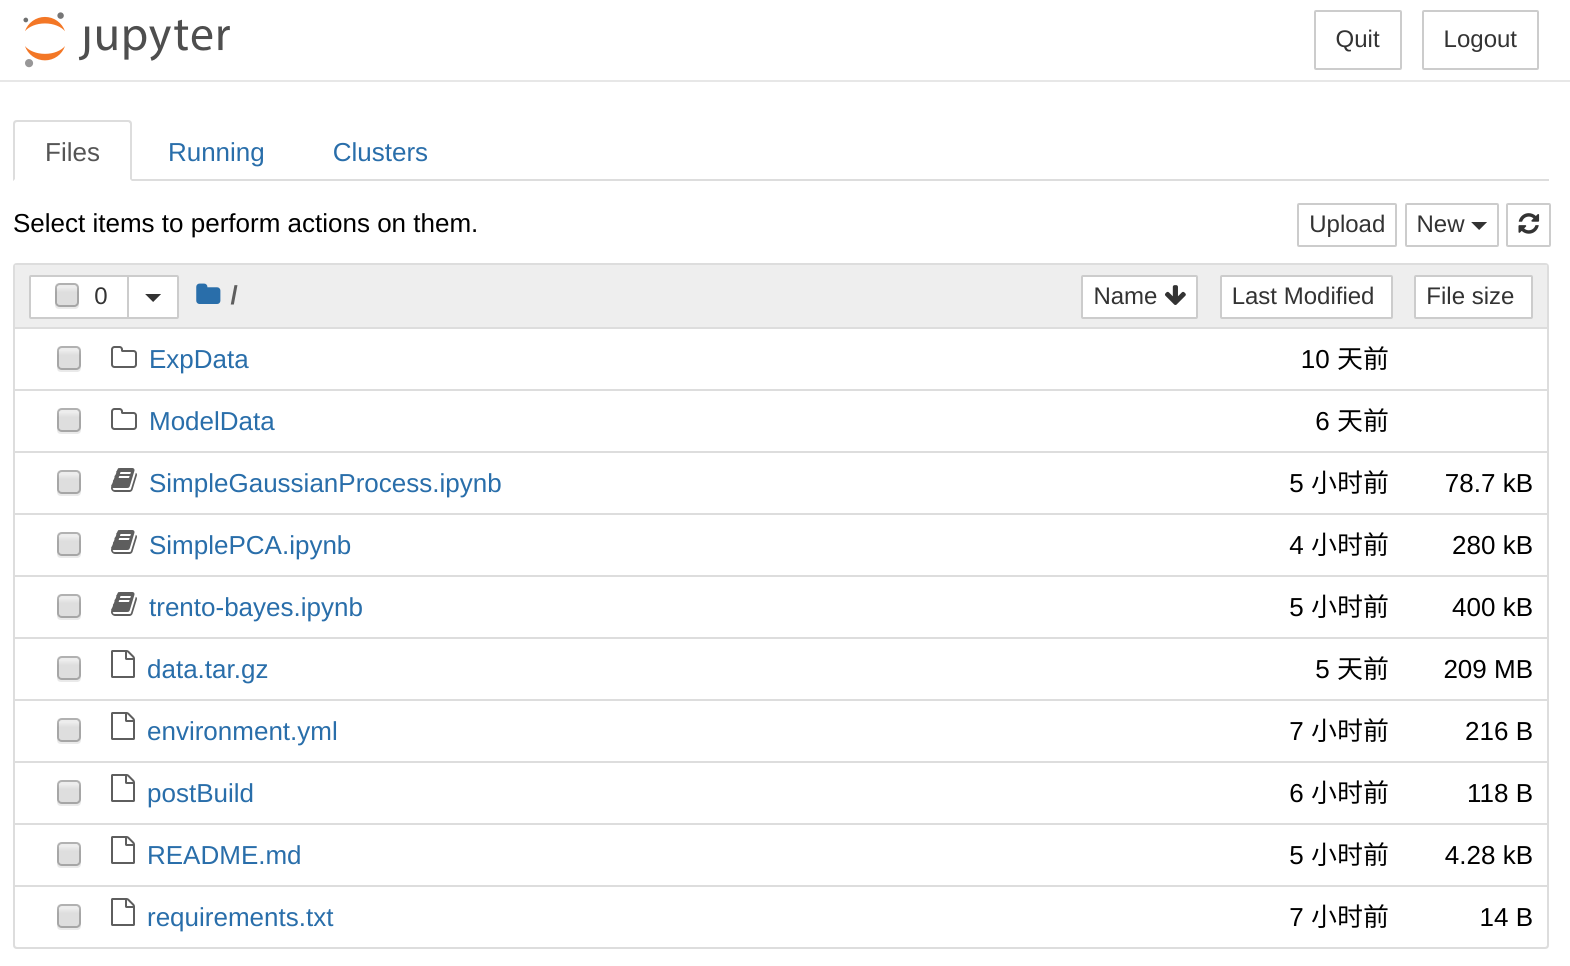
\includegraphics[width=.6\textwidth]{figs/Notebook-1.png}
\end{center}
\end{frame}

\begin{frame}{Load and test the libraries}
Open the notebook ``trento-bayes.ipynb". Run the code blocks by pressing ``Shift+Enter". Check if you can run the following block that loads all the modules to be used in the exercises.

\begin{center}
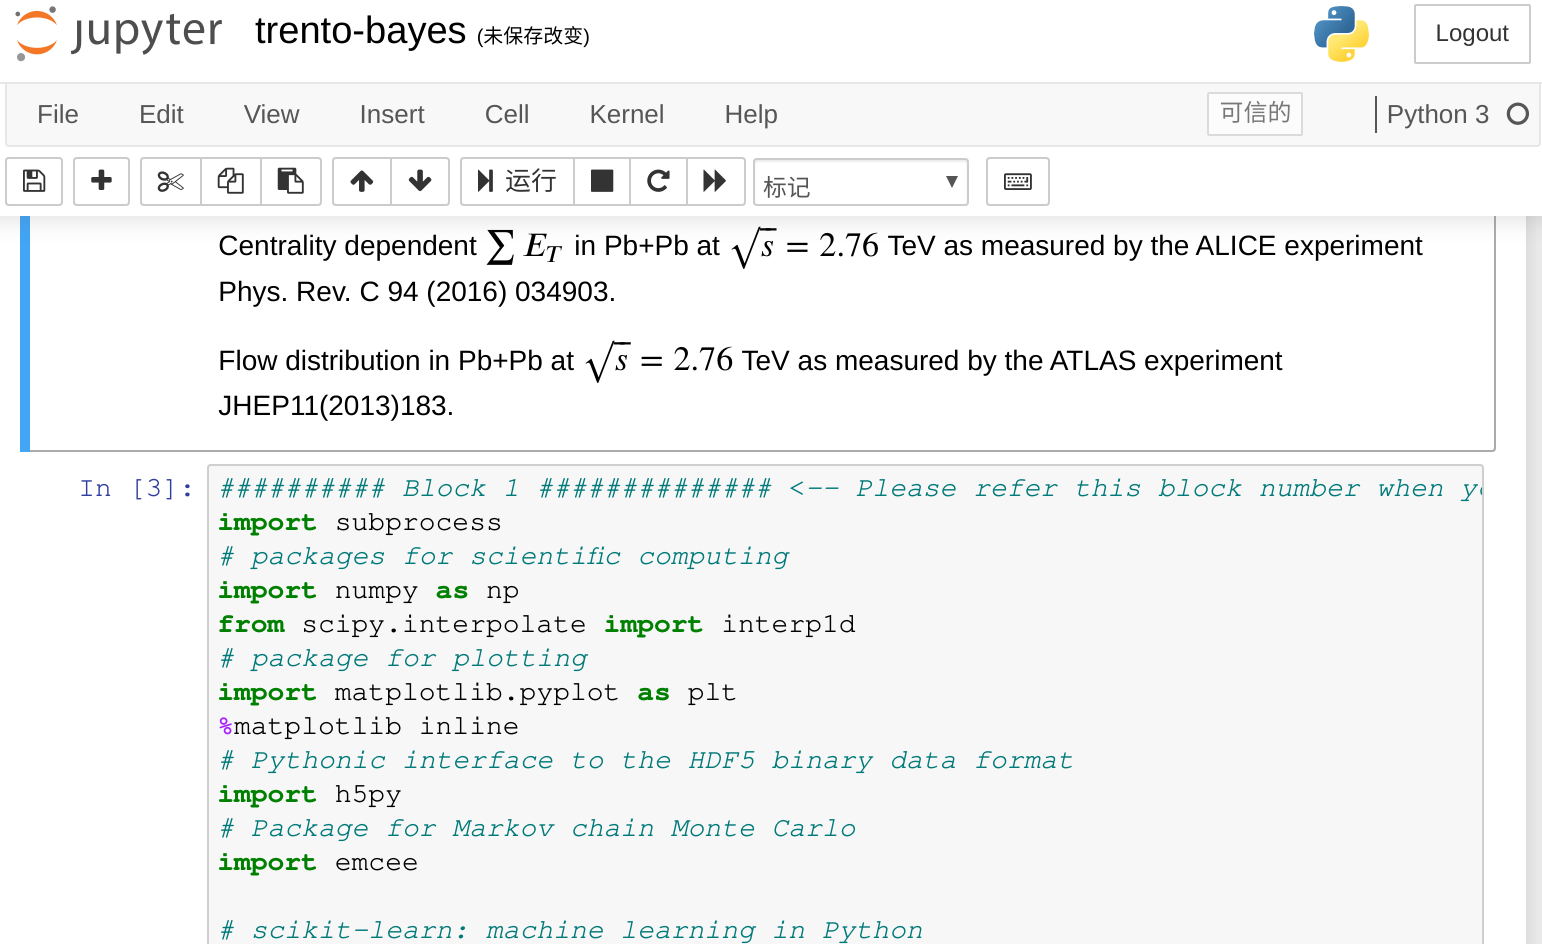
\includegraphics[width=.7\textwidth]{figs/load.png}
\end{center}
\end{frame}

\end{document}